\chapter{Design}
% input Design sections for no auto new page
This chapter describes the design of a MIPS 1 microcontroller. The microcontroller design is shown \autoref{fig:overview}.

\begin{figure}[h]
\centering{
\resizebox{100mm}{!}{\input{design.pdf_tex}}
\caption{CPU overview}
\label{fig:overview}
}
\end{figure}

The CPU is divided in a control and a datapath blocks. In the datapath there is the pipeline made of five blocks:
\begin{itemize}
 \item IF: Instruction fetch
 \item ID: Instruction decode
 \item Ex: Execution
 \item Me: Memory stage
 \item WB: Writeback
\end{itemize}

The CPU interacts with two external memories and has also a clock and a reset input.
\section{ALU}
This section describes the ALU (arithmetic logic unit). The implementation of the ALU has three parallel data buses consisting of two 32bit input operands and a 32bit result output.
Furthermore, there is an 6bit input for the opcode. The ALU can perform 7 operations: add, sub, and, or, sll, slt and interconnect one of the two inputs to the result output. 
Additionally, there is an zero output flag if the operation results in zero.

\begin{figure}[h!]
  \centering
  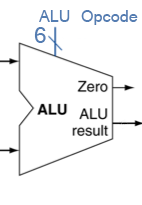
\includegraphics[width=0.3\textwidth]{figure/alu.png}
  \caption{ALU}
  \label{fig:ALU}
\end{figure}

	\section{Datapath}
This section describes the data-path and its internal elements. The data-path is the component that connects the pipeline components within itself as well as with CPU inputs and outputs and the control-path.

This MIPS implementation works with a 5 stage pipeline in order to achieve a fast clock. The data-path consists of instruction fetch, instruction decode, execution, memory stage and write-back.
The data-path controls the information flow from one pipeline stage to the next with registers. 
These writing process occur on the positive edge of the clock when the pipeline stage input from the control-path, so that the registers forwards information synchronously. 
The data-path forwards the control-path signals asynchronously, contrary to the pipeline to pipeline signals.



\begin{figure}[h!]
  \centering
  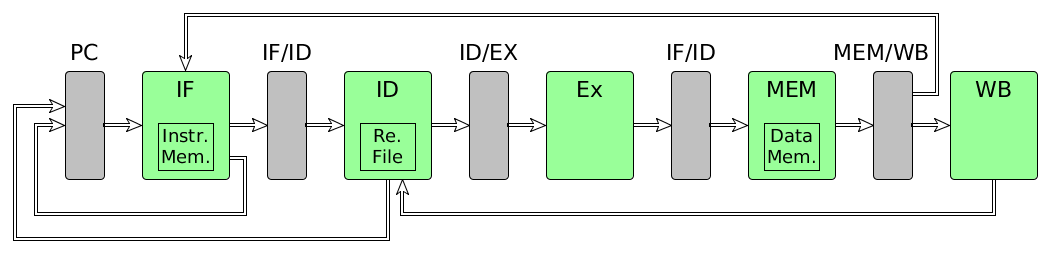
\includegraphics[width=0.8\textwidth]{figure/datapath.png}
  \caption{Data-path pipeline}
  \label{fig:datapath}
\end{figure}

The program counter (PC) is programmed into the data-path. Its function is the store the current program address, which is mostly counted up.
It has a multiplexer controlled by the control-path to choose the input. The two possible inputs are to count up (PC+4) from instruction fetch
and the jump or branch from instruction decode. The control-path chooses always the instruction decode input in the case of jump or branch. 


The following subsections describe the pipeline components as well as its functions and IOs. 

\subsection{Instruction fetch}
This first block of the pipeline is the instruction fetch. The main task of this block is to fetch the next instruction and relay it to the pipeline. 

The program counter is a 32-bit input, which is directly outputted as instruction address to fetch an instruction. The instruction fetch inputs the program memory's instruction data, 
with the 32-bit instruction. This value is directly forwarded to the pipeline. The memory word is one byte long, but each instruction read operation retrieves four bytes or the 32-bit
word.

The program counter is also incremented by four, because the used memory is 8-bit long, pointing to the next valid instruction. This incremented value is given back to PC.
\subsection{Instruction decode}
The second block of the pipeline if the instruction decode. Its main tasks are to divide the instruction into its pieces, manage the register file and manage branches.

The main input is the instruction from the instruction fetch stage. This instruction is 32-bit long and can be of three types. These are shown in \autoref{tab:instr type} \cite{mips32}.

\begin{table}[h!]
	\centering
	 \caption{MIPS instruction types}	
	\begin{tabular}{ccccccc}
		\toprule[2pt]
		\textbf{Type} & \multicolumn{6}{c}{\textbf{format (bits) }}   \\
		\toprule[2pt]
		R & opcode (6) & rs (5) & rt (5)   & rd (5) & shat (5) & funct (6) \\
		I & opcode (6) & rs (5) & rt (5)   & \multicolumn{3}{c}{ immediate (16)} \\
		J & opcode (6) & \multicolumn{5}{c}{ address (26)} \\	
		\bottomrule[2pt]
	\end{tabular} 
	\label{tab:instr type}
\end{table}

The \textbf{opcode} indicates the operation or arithmetic family of operations. Opcode equals zero are the R-type operations. The field \textbf{funct} provides an specific operation.
\textbf{rs}, \textbf{rt} and \textbf{rd} provide sources or destinations register addresses. \textbf{shamt} indicates the shift amount for shift operations. \textbf{immediate} carries
a relative address or constant, which is zero or sign extended to 32-bits. \textbf{address} is an absolute address.

The main outputs are register A, register B, shift, regdest, immediate and IP. Other than IP, all outputs depend on the instruction decoding. 
Register A contains always the value that is contained in the register given by the source register field (instruction's sub-vector 25-21). 
Register B likewise always contains the value of the register given by the R-type-instruction's field for the target register (instruction's sub-vector 20-16). 
Immediate always contains the lower half of the instruction with a signed extension. 

Regdest has to be chosen by the control path. It can be either the target 
register field or the R-type's destination register field or 31, which was originally implemented for jump-and-link- or branch-and-link-instructions, but rendered pointless
by the more complex branch logic and write-back functionality for register 31. Shift also must be chosen by the control path. It can be set to the R-type-instruction's shift-field, 
to 16 or to 0. 

The execution stage chooses the signals necessary for an operation using two multiplexers so if any output yields a nonsensical value is is simply not used.

\subsubsection{Register File}
The register file is a set of 32 general purpose 32-bit registers. These have the advantage, comparing to the ram memory, that they can always be accessed within one clock cycle.
The access to these registers is made with five bits, which allows multiple registers to be referenced per instruction. All loaded memory values are stored in a register
for later use.

The registers are numbered from \$0 through \$31. There is also a convention for using these registers, which must be enforced by assembly language and follow \autoref{tab:mips registers} 
\cite{regfiles}:

\begin{table}[h!]
	\centering
	 \caption{MIPS registers}	
	\begin{tabular}{ccl}
		\toprule[2pt]
		\textbf{Register Number} & \textbf{Conventional Name} &\textbf{Usage}  \\
		\toprule[2pt]
		\$0 & \$zero & Hard-wired to 0 \\
		\$1 & \$at & Reserved for pseudo-instructions \\
		\$2 -\$3 & \$v0, \$v1 & Return values from functions \\
		\$4 - \$7 & \$a0 - \$a3 & Arguments for functions - not preserved by subprograms \\
		\$8 - \$15 & \$t0 - \$t7 & Temporary data, not preserved by subprograms \\
		\$16 - \$23 & \$s0 - \$s7 & Saved registers, preserved by subprograms \\
		\$24 - \$25 & \$t8 - \$t9 & More temporary registers, nor preserved by subprograms  \\
		\$26 - \$27 & \$k0 - \$k1  & Reserved for kernel. Dot not use. \\
		\$28 & \$gp & Global Area Pointer (base of global data segment) \\
		\$29 & \$gp & Stack pointer \\
		\$30 & \$sp & Frame Pointer \\
		\$31 & \$ra & Return Address \\
		\bottomrule[2pt]
	\end{tabular} 
	\label{tab:mips registers}
\end{table}

This implementation of MIPS does not have a FPU. In case of FPUs another 32 32-bit register set is used.

The register file is written on the clock's negative edge with write-back information. The register file require a 5-bit destination register address and the 32-bit word to be written into the register. 
Additionally there is the possibility to write to register 31. On every rising clock cycle, an internal write-back flag is checked. If it was set by another process, 
the value of the internal write-back register is copied to register 31. This bypasses some pipeline stages, but makes control path design a little easier.
\subsubsection{Branch Logic}
The branch and jump instructions require just one clock between instruction fetch and the jump itself. Due to this constrain, there is the need of a branch logic inside
the instruction decode part. The output of this operation is the next instruction address for PC. 

On the jump command, PC will receive the jump value. 
In case of a branch, PC will receive either the branch value or PC+4, depending on the instruction decode decision. This behavior allows for the control-path always to 
activate the instruction decode input in cases of jumps and branches. If a Jump-and-link- or a branch-and-link-instruction is detected, the branch logic writes the last 
program counter to the internal write-back register and sets the internal write-back flag to 1 to signal a necessary copy operation to the register bank. 
It evaluates the flag and treats the internal write-back register as described above.
\subsubsection{Forwarding}
Often calculated or memory read values are used in the following instructions. Due to the pipeline, the values are not ready in the register file, causing a data hazard. In order to avoid this conflict
a data forwarding system is integrated. The data forwarding provide separated inputs for the 5-bit destination register address and the 32-bit word for the ALU, memory stage and write-back. 
If the destination register address in one of this stages is equal to an address used in the current instruction decode phase, the value of the register bank is replaced by a forwarded value. 
The forwarding system takes care to always use the most recent value. For example, if both write-back and execution stage contain the same destination address, 
the execution stage's value is forwarded because the value that has to be written to that destination register was changed by the instruction in the execution stage after 
it was changed by the instruction in the write-back stage, so the value contained in the execution stage is the most recent.


\subsection{Execution}
This stage of the pipeline takes care of the actual mathematical operations. It provides two main multiplexers, one for each value input of the ALU.
The inputs of the first multiplexer are the zero padded shift input, the number four (32-bit) and the register A from instruction decode. The second multiplexer provides register B, 
the immediate value and IP as inputs.

Both multiplexers are controlled by the control-path.
\subsection{Memory Stage}
The memory stage is the fourth block of the pipeline and has the main task of fetch or save in the memory. 

For memory operations the execution stage outputs two 32-bit values: aluResult\_in, which works as the memory address, and data\_in, which is data to be written in the memory. 
On read operations, the data\_to\_cpu input delivers the 32-bit memory value.

This stage has one multiplexer choosing the pipeline stage output from aluResult\_in or data\_to\_cpu.
\subsection{Write-back}
This write-back stage is the fifth and last stage of the pipeline. Its main task is just to hold the calculated values, as well as the values read from the memory 
so they can be written the register file.

	\section{Controlpath}
The control path is not designed as a finite state machine. Due to its simplicity we chose an approach that is closer to the pipelined structure of the MIPS-Architecture. The control path is built around a 32-bit wide 4-deep shift register. When the memory returns the instruction to the instruction-decode-stage of the datapath, it is also fed into the shift register and propagates in the following clock cycles. To the stages of this shift register we attatched a decoder that produces control signals for one stage of our datapath. Each stage of the shift register matches exactly one stage of the datapath, except for the first controller stage which handles instruction fetch and instruction decode. The second stage returns the control signals for the execution stage, the third stage is mapped to the memory stage and the fourth stage controls the datapath's writeback stage. In case of any stalls the propagation of the instructions through the shift register is halted.
\subsection{Decoder for the instruction-fetch- and instruction-decode-stage}
The decoder attatched to the first stage of the shift register distinguishes between the opcodes of the given instruction to determine the control signals. If the opcode is 000000, an R-type-instruction is assumed and the instruction-decode-stage's destination register control signal is set to 0 to use the R-type destination register. The shift multiplexor is set to 0 as well to use the R-type-instructions shift field. For the settings of the pc's multiplexor in the instruction-fetch-stage, the other bits of the instruction are evaluated. If they make the instruction a Jump-Register-instruction, the signal is set to 1 so that the new program counter calculated by the branch logic is used instead of the previous value incremented by 4. In every other case, this multiplexor's control signal is set to zero because all other R-type-instructions do not modify the program counter.\\
All non-R-type-instructions are treated as I-type-instructions by the decoder. This means, that the control signal for the shift-multiplexor is set to 0 for all instructions except the LUI-Instruction, which needs a shift of 16. Therefore, the signal is set to 1. A more complex decision has to be made for the program counter multiplexor. All instructions that influence the program's control flow (Branch- and Jump-Instructions) produce an output of 1, all other instructions return 0 and the program counter is incremented by 4. The multiplexor for the destination register is always set to 2 to use the I-type-instruction destination field. This is again ignored, when a J-type-instruction reaches the further stages, so no damage is done.
\subsection{Decoder for the execution-stage}
The decoder for the execution stage has to set the signals that select the operands of the operation to be executed and set the kind of operation the ALU has to perform. Since the instruction's opcode is in hardly any way connected to the executed operation, the decoder logic is a little more difficult. It groups all operations of the example code that perform an addition of a register's value to the immediate value of the instruction (ADDIU, LW, SW, SB, LBU) and sets the control signals to 2 for the ALU's a-operand, 1 to forward the immediate field to the ALU and the ALU's operation code itself is set to 20 for addition. For the LUI-instruction, the ALU's a-operand-multiplexor is set to 0 for a shift of 16, the b-operand-multiplexor is set to 1 for the immediate-field and the ALU itself is perfoming the shift operation. All other immediate-operations get the a-operand-multiplexor set to 2, b set to 1 and the ALU operation code set according to the instruction. The only supported R-type operation, SLT gets a set to 2, b set to 0 and the ALU set for set-less-than-operations. All other R-Type instructions are treated like NOOP-instructions: A set to 2, b set to 0 and the ALU-operation set to a left-shift. Although the datapath would be able to support more operations, the datapath is limited to the described instructions and has to be expanded for a full MIPS instruction set.
\subsection{Decoder for the memory stage}
The memory stage's decoder is more simple than the execution stage's decoder. It just has to evaluate whether the instruction is a store-instruction, a load-instruction or any other instruction. In case of a load instruction the multiplexor signal for the memory access has to be set to 1 to let the result of the memory access get to the writeback stage. In all other cases, this signal is set to 0 to just forward the signal coming from the execution stage. The read or write masks are set according to the instruction stored in the shift register stage. A SW-instruction for example produces an output of F for the write mask and an LBU-instruction returns a read mask of 1. All other instructions have read and write masks of 0.
\subsection{Decoder for the writeback stage}
The decoder for the writeback stage is the simplest of the whole controller because it controlls just one signal that enables the register bank. It distinguishes between the commands that write back to the register bank bank (currently supported: LUI, ADDIU, LW, LBU, SLTI, SLT, ANDI, ORI) and sets the \em enable_regs\em -signal to for them, and the other instructions, where the register bank is disabled by setting the signal to zero. 